\begin{sectionbox}
    \subsection{Rexlexion und Brechnung}
    $f_{\text{Medium}}\lambda_{\text{Medium}} = c_{\text{Medium}} \qquad \lambda_{\text{Medium}} = \frac{\lambda_{\text{Vakuum}}}{n}$\\
    Berchnungsindex $n=\frac{c_\text{Vakuum}}{c_{\text{Medium}}}$
    \subsubsection{Brechung}
    \begin{emphbox}
        \textbf{Gesetz von Snellius:}
        $\frac{\sin \alpha}{\sin \beta} = \frac{n_2}{n_1} = \frac {c_1}{c_2}$
    \end{emphbox}
    \begin{enumerate}
        \item[A)] \textbf{zum Lot} (dünn nach dicht)\\
              $\sin \alpha > \sin \beta$ \qquad $c_1 > c_2$
        \item[B)] \textbf{vom Lot} (dicht nach dünn)\\
              $\sin \alpha < \sin \beta$ \qquad $c_1 < c_2$
    \end{enumerate}
    \subsubsection{Totalreflexion}
    Nur möglich wenn $n_1 > n_2$ und $\theta > \theta_{\ir krit}$ \\
    $\theta_{\ir krit} = \arcsin \frac{n_2}{n_1}$\\
    Einfallswinkel = Ausfallswinkel
\end{sectionbox}

\begin{sectionbox}
    \subsection{Linsen}
    \begin{tablebox}{ll}
        Linsengleichung &
        $D=\frac{1}{f}=\frac{1}{g}+\frac{1}{b}$\\
        Vergößerung & $V=\frac{B}{G}= - \frac{b}{g}=\frac{\tan \alpha}{\tan \alpha_0}$\\
    \end{tablebox}
    $g>0$ links der Linse, $b>0$ rechts der Linse \\
    Falls $b<0 \Rightarrow$ virtuelles Bild \\
    Falls $V < 0$: Bild nach unten geklappt \\
    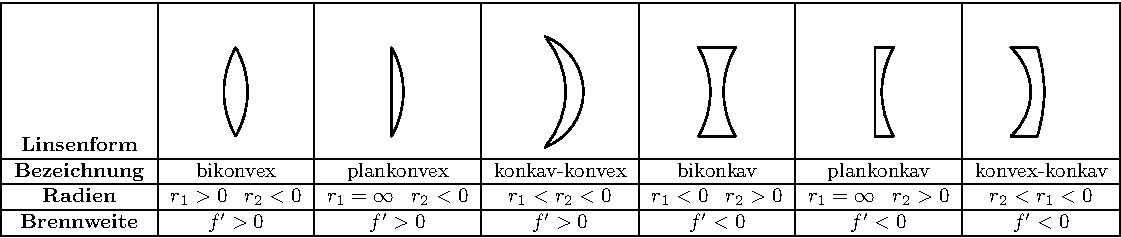
\includegraphics[width=\columnwidth]{img/Linsen_crop.pdf}

    \subsubsection{Hohlspiegel}
    $f=\frac{r}{2}$ \qquad $V=\frac{B}{G}= - \frac{n_1b}{n_2g}$ \\
    $D=\frac{n_1}{g}+\frac{n_2}{b}=\frac{n_2-n_1}{r}$\\
    $g\rightarrow \infty: b=f_B=\frac{n_2r}{n_2-n_1}$\\
    $b\rightarrow \infty: g=f_G=\frac{n_1r}{n_2-n_1}$\\

    \subsubsection{Dünne Linsen}
    $\frac{1}{f}=\frac{1}{g}+\frac{1}{b}=(\frac{n_2}{n_1}-1)(\frac{1}{r_1}-\frac{1}{r_2})$\\
    mit $r_1$ Krümmungsradius der linken Linse, $r_2$ Krümmungsradius der rechten Linse (bei rechtskonvex ist $r_2<0$)

    \paragraph{Konvexe Linse (Sammellinse)}
    Korrektur von Weitsichtigkeit \\
    $V_{\ir sammel}= \frac{b}{g}=\frac{b-f}{f}$\\

    Abbildung:
    \begin{tablebox}{lcllr}
        $\infty > g > 2f $ & $\Rightarrow$ & $2f>b>f$ & $G>B$ & real und invertiert\\
        $g=2f $ & $\Rightarrow$ & $2f=b$ & $G=B$ & real und invertiert\\
        $2f>g>f $ & $\Rightarrow$ & $ \infty >b>2f$ & $G<B$ & real und invertiert\\
        $0<g<f $ & $\Rightarrow$ & $ -b>g$ & $G<B$ & virtuell und aufrecht\\
    \end{tablebox}
    \paragraph{Konkave Linse (Zerstreuungslinse)}
    Korrektur von Kurzsichtigkeit\\
    Abbildung:
    \begin{itemize}
        \item[$\rightarrow$] Bild immer zwischen Brennpunkt und Linse
        \item[$\rightarrow$] Bild immer verkleinert ($G>B$)
        \item[$\rightarrow$] Bild immer virtuell und aufrecht
    \end{itemize}

    \subsubsection{Dicke Linsen}
    $\frac{1}{f}=(\frac{n}{n_0}-1)\cdot(\frac{1}{r_1}-\frac{1}{r_2}+\frac{(n-n_0)d}{n \cdot r_1 r_2})$\\
    $h_1=-\frac{f(n-1)d}{n \cdot r_2}$ \qquad $h_2=-\frac{f(n-1)d}{n \cdot r_1}$

    \subsubsection{Linsensysteme}
    \begin{itemize}
        \item \textbf{Lochkamera} \\
              $S=\frac{D(b+g)}{g}$
        \item \textbf{Lupe} \\
              $V=\frac{\tan \alpha_L}{\alpha_0}=\frac{G/f}{G/s_0}=\frac{s_0}{f}$ mit $s_0=\SI{25}{\centi \meter}$
        \item \textbf{Fernrohr} \\
              $V=\frac{f_{ob}}{f_{ok}}$, $g\approx \infty$, $b\approx f$ \\
              $V_T=\frac{f}{g-f}=\frac{b-f}{f}\approx 0$
        \item \textbf{Mikroskop} \\
              $V=V_{ok}\cdot V_{ob}=\frac{(d-f_{ob})s_0}{f_ob \cdot f_ok}=-\frac{l}{f_{ob}}\cdot \frac{s_0}{f_{ok}}$
        \item \textbf{Auflösung Mikroskop} \\
              mit Spalt b: $\delta_{\ir{min}} = \alpha = \arcsin\frac{\lambda}{b} \approx \frac{\lambda}{b}$ (Abbé Limit)\\
              für runde Linse mit Durchmesser D: $\delta_{\ir{min}} = D\cdot\sin\alpha = 1,22\frac{\lambda}{D}$ (Rayleigh-Kriterium)\\
    \end{itemize}
\end{sectionbox}

\begin{sectionbox}
    \subsection{Absorption}
    Berchungsindex mit Absorption: $n\rightarrow \tilde{n}=n-i\kappa$\\
    Re($\tilde{n}$)$=n$: Brechung \\
    Im($\tilde{n}$)$=\kappa$: Absorption \\

    \begin{emphbox}
        \textbf{Absorptionsgesetz} von Lambert-Beer: $I=I_0e^{-\alpha \cdot d}=I_0e^{-\frac{2\omega}{c}\kappa d}$
    \end{emphbox}

    \subsubsection{Polarisation}
    \begin{emphbox}
        \textbf{Gesetz von Malus} (für polarisiertes Licht): $I = I_0 \cos^2 \alpha$
    \end{emphbox}
    Für unpolarisiertes Licht gilt nach einem Polarisationsfilter: $I = \frac{I_0}{2}$
\end{sectionbox}
